\begin{frame}
    \begin{figure}
        \hspace*{-320pt}
\includegraphics[width=1.0cm]{vstu_logo}
    \end{figure}
    \vspace{2em}
    \begin{center}
        \large
        \textbf{Метод построения маршрутов общественного транспорта на основе предпочтений жителей}\\
    \end{center}
    \vspace{2em}
    \begin{flushleft}
        \hspace{12em}Автор:~Голубев~А.~В.\\
        \hspace{12em}группа:~САПР-2п1\\
        \hspace{12em}Руководитель:~Щербаков~М.~В.
    \end{flushleft}
    \vspace{3em}
    \centeringВолгоград \the\year\ г.
\end{frame}

\begin{frame}
    \frametitle{Цели и задачи}
    \textbf{Целью} данной работы являлось разработка метода генерации маршрутов общественного транспорта на 
    основе предпочтений жителей для минимизации дискомфорта перемещения в городе.

    В данной работе рассматриваются к решению следующие задачи:
    \begin{itemize}
        \item разработка метода построения маршрутной сети между кластерами предпочтений;
        \item модификация и использование существующих алгоритмов для задачи маршрутизации;
        \item разработка критериев оценки качества построенных маршрутов;
        \item представление построенных маршрутов на карте.
    \end{itemize}
\end{frame}

\begin{frame}
    \frametitle{Актуальность}
    Изменения в городской среде требуют формирования новых механизмов планирования инфраструктуры города. 
    Для получения эффективных результатов, следует осуществлять принятие решений на основе актуальных 
    данных, отражающих предпочтения жителей.
    \begin{figure}
        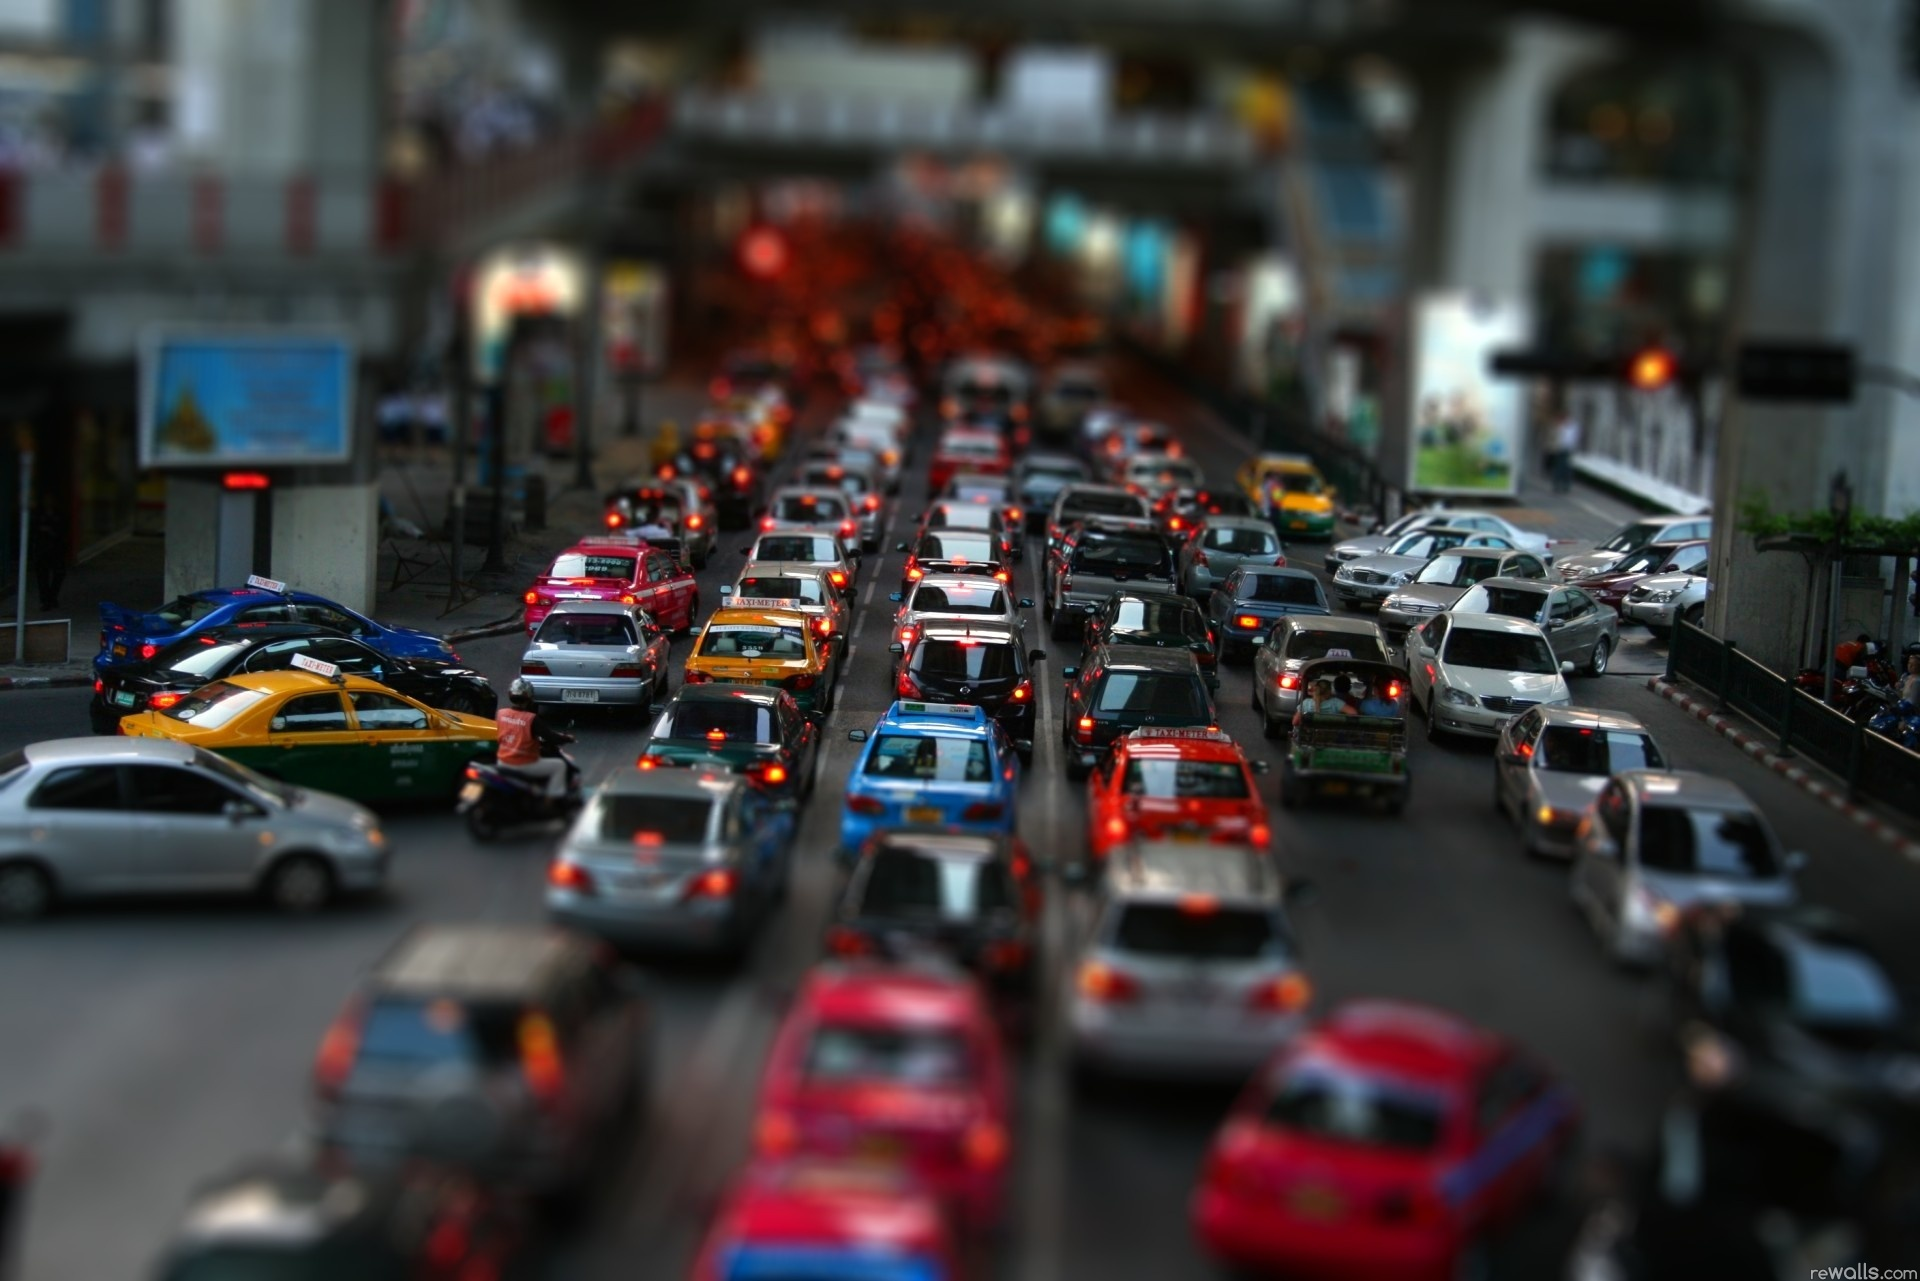
\includegraphics[width=0.7\textwidth]{traffic-jam}
    \end{figure}
\end{frame}

\begin{frame}
    \frametitle{Анализ предметной области}
    Существующие инструменты для проведения комплексного анализа:
    \begin{itemize}
        \item Citilabs Cube Cloud;
        \item PTV Visum;
        \item INRO Emme;
        \item TRANSIMS;
    \end{itemize}
    \begin{figure}
        \centering
        
\includegraphics[width=0.1\textwidth]{cube-cloud-logo}\quad
        
\includegraphics[width=0.2\textwidth]{ptv-visum-logo}\quad
        
\includegraphics[width=0.3\textwidth]{inro-emme-logo}\quad
        
\includegraphics[width=0.25\textwidth]{transims-logo}
    \end{figure}
\end{frame}

\begin{frame}
    \frametitle{Постановка задачи}
    \textbf{Объект исследования} -- построения маршрутов общественного транспорта на основе актуальных 
    данных о предпочтениях жителей по перемещению в современной городской среде.\\\vspace{1em}

    \textbf{Предмет исследования} -- разработка и применение методов построения маршрутов 
    общественного транспорта учитывающие актуальные данные о предпочтениях жителей.\\\vspace{1em}

    \textbf{Гипотеза исследования} -- существующие системы используемые для анализа и построения маршрутных 
    сетей городского транспорта не учитывают данные о предпочтении жителей по перемещении.
\end{frame}

\begin{frame}
    \frametitle{Предлагаемые методы для решения задачи}
    \small
    \begin{itemize}
        \item \textbf{Методы локального поиска} --- вероятность <<свалиться>> в локальный оптимум.
        \item \textbf{Поглощающий алгоритм} --- игнорирование локально неоптимальных решений влияющих на 
            конечный результат.
        \item \textbf{Метод поиска чередующихся окрестностей} --- получение локально оптимального решения.
        \item \textbf{Метод имитации отжига} --- подбор начальных значений и введение ограничений зависящих 
            от них.
        \item \textbf{Поиск с запретами} --- необходимо введение параметра отвечающий за число итерация, 
            для предотвращения зацикливаний алгоритма.
        \item \textbf{Семейство генетических алгоритмов} --- представление графа сети в виде хромосом и 
            выбор <<хорошей>> функции приспособления.
    \end{itemize}
\end{frame}

\begin{frame}
    \begin{figure}
        \centering
        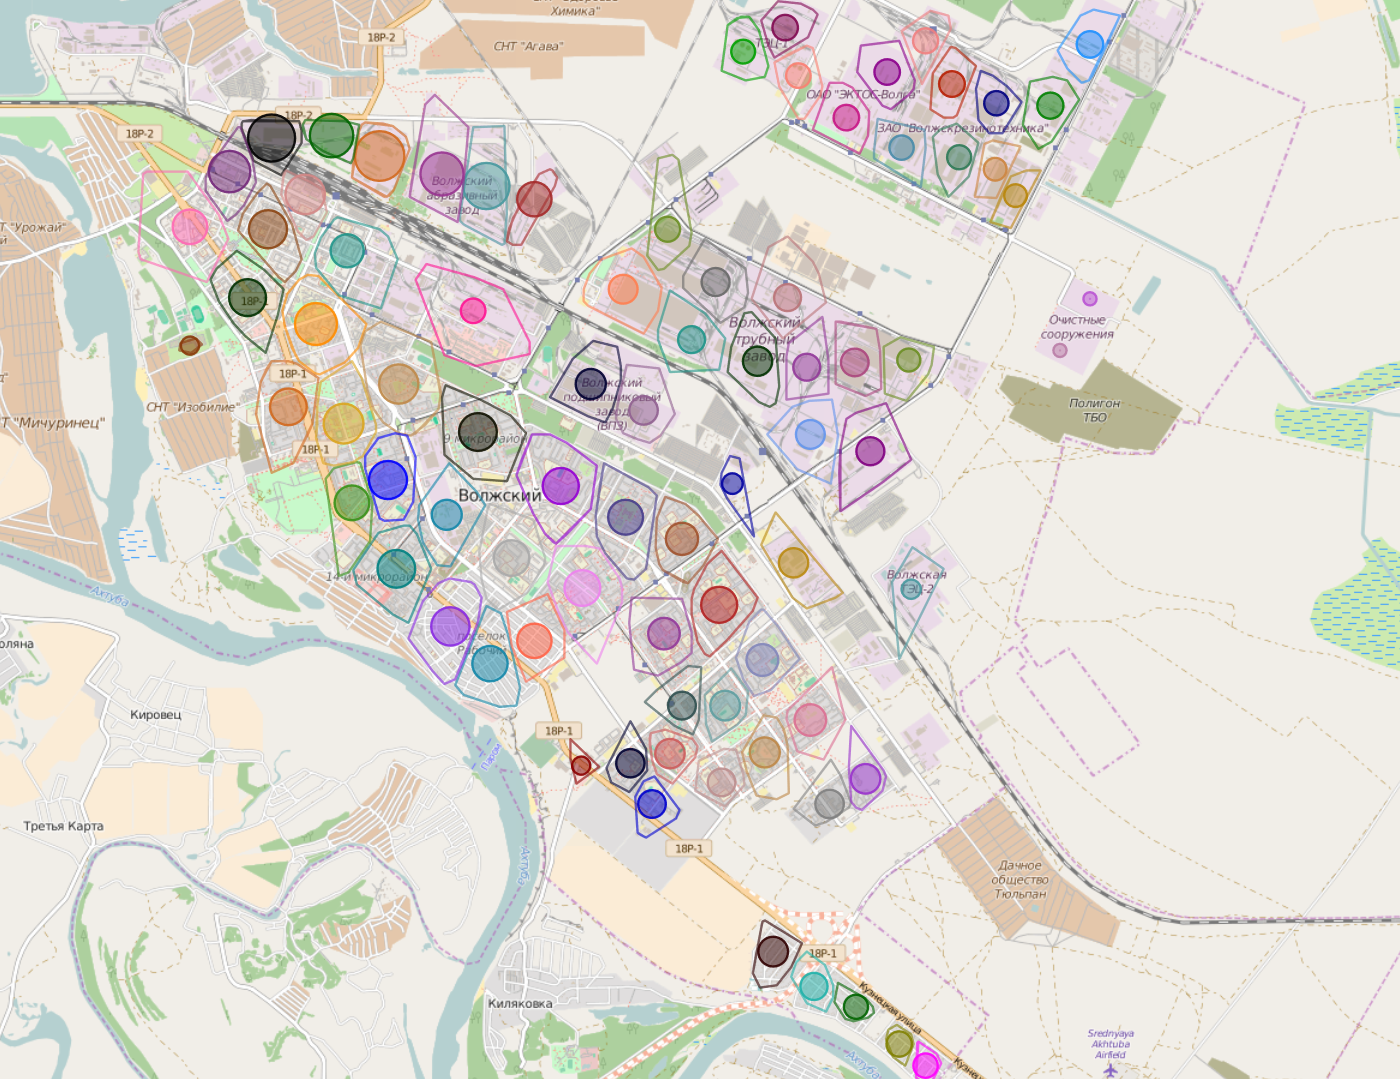
\includegraphics[width=\textwidth]{test-clustered-data}
    \end{figure}
\end{frame}

\begin{frame}
    \frametitle{Алгоритм выбора кластеров}
    \begin{figure}[ht!]
        \scriptsize
        \begin{algorithm}[H]
            \KwData{\( n_r \) -- количество маршрутов для построения (подбирается с учетом конкретной задачи), 
                \( G \) -- список вершин исходного графа.}
            \KwResult{\( C_t \) -- список терминальных вершин, \( C_{nt} \) -- список нетерминальных вершин.}
            1) Рассчитать координаты центра \( r_0 \) окружности, охватывающей все вершины графа \( G \) 
                (складываем покомпонентно координаты узлов и делим полученные значения на количество узлов)\;
            2) Сформировать список \( D \) расстояний от \( r_0 \) до каждой вершины \( c_j \)\;
            3) Найти вершину с максимальным удалением от центра окружности и построить окружность с радиусом 
                равным расстоянию до этой вершины\;
            4) Разбить окружность на \( 2\cdot n_r \) равных отрезков и поместить значения полученных 
                углов (в полярной системе координат) в \( N_c \)\;
            5) Обойти список \( N_c \) и получить координаты точек на окружности по углу и радиусу с 
                использованием проекции Меркатора, и поместить полученные значения координат вершин в 
                список \( C_t \)\;
            6) \ForEach{элемента \( c_j \) из \( C_t \)}{
                6.1) Найти узлы в окрестности \( \varepsilon \), добавить в список \( T \)\;
                6.2) Выбрать из списка \( T \) вершину \( c_k \) с максимальным весом\;
                6.3) Заменить \( c_j \) на \( c_k \)\;
            }
            7) Составить список \( C_{nt} \) из вершин не входящих в список \( C_t \)\;
        \end{algorithm}
    \end{figure}
\end{frame}

\begin{frame}
    \frametitle{Алгоритм построения сети маршрутов}
    \begin{figure}[ht!]
        \footnotesize
        \begin{algorithm}[H]
            \KwData{\( n_r, C_t, C_{nt} \)}
            \KwResult{\( R_i \) -- список маршрутов сети.}
            1) Создать сеть \( R_i \) соединяющий вершины \( C_t \)\;
            2) \ForEach{\( i \)-го маршрута из сети \( R_i \)}{
                2.1) Поместить вершины маршрута (попарно) в список \( PN \)\;
                2.2) Найти вершину \( c_j \) (из \( C_{nt} \)), присоединение которой минимально увеличивает 
                    длину маршрута из \( PN \) и добавить новый маршрут в список \( RC \)\;
                2.3) Составить новый список \( RCC \) состоящий из маршрутов, полученных путём замены пар 
                    вершин \( PN \) на изменённые \( RC \)\;
                2.4) Рассчитать длины маршрутов в списке RCC, используя OSRM\;
                2.5) Выбрать из \( RCC \) маршрут \( R^{\star}_i \) с минимальной длиной\;
                2.6) Заменить \( R_i \) на \( R^{\star}_i \)\;
                2.7) Удалить узел \( c_j \) из \( C_{nt} \) добавленный в \( R^{\star}_i \)\;
            }
            3. Если список \( C_{nt} \) не пустой, перейти на шаг 2, иначе закончить построение\;
        \end{algorithm}
    \end{figure}
\end{frame}

% Проектирование программного продукта (два слайда) 
% Написать архитектуру ПО

\begin{frame}
    \frametitle{Проектирование программного продукта}
    Программное обеспечение должно обеспечивать возможность выполнения следующих функций:
    \begin{itemize}
        \item построение матрицы корреспонденций по данным о перемещении;
        \item анализ графа корреспонденций для выбора узлов отправления-назначения;
        \item построение маршрутной сети по заданным параметрам;
        \item оценка построенной маршрутной сети по критериям;
    \end{itemize}
\end{frame}

\begin{frame}
    \frametitle{Проектирование программного продукта}
    \small
    Используемые технологии:
    \begin{itemize}
        \item Python 3 (\url{https://www.python.org/})
        \item OSRM (\url{http://project-osrm.org/})
        \item OpenStreetMap (\url{https://www.openstreetmap.org})
        \item Leaflet (\url{http://leafletjs.com/})
    \end{itemize}
    Исходный код доступен по следующей ссылке:\\
    \url{https://github.com/vstu-cad-stuff/routing/tree/master}\\\vspace{1em}
    Результаты работы реализованных алгоритмов:\\
    \url{https://vstu-cad-stuff.github.io/routing/}
\end{frame}

\begin{frame}
    \frametitle{Научная новизна}
    Научная новизна работы обусловлена:
    \begin{itemize}
        \item предложена автоматизация процесса построения начальной маршрутной сети без участия 
            транспортного инженера;
        \item предложен метод основанный на использовании данных о предпочтении жителей для построения 
            сети маршрутов общественного транспорта;
        \item разработан метод построения сети маршрутов общественного транспорта.
    \end{itemize}
\end{frame}

\begin{frame}
    \frametitle{Результат}
    \framesubtitle{Евклидова метрика в проекции Меркатора}
    \begin{figure}[ht!]
        \centering
        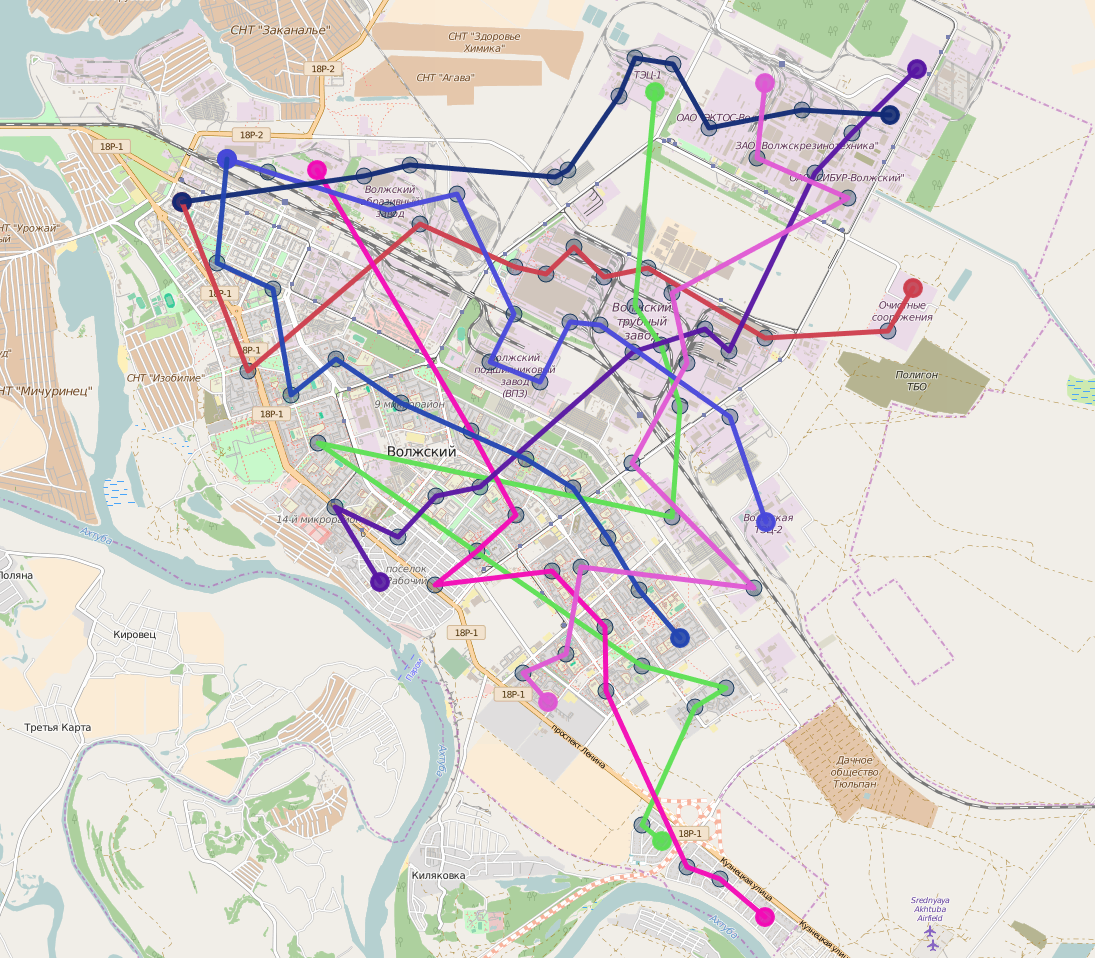
\includegraphics[width=0.8\textwidth]{100-8}
    \end{figure}
\end{frame}

\begin{frame}
    \frametitle{Результат}
    \framesubtitle{Построение по дорожной сети}
    \begin{figure}[ht!]
        \centering
        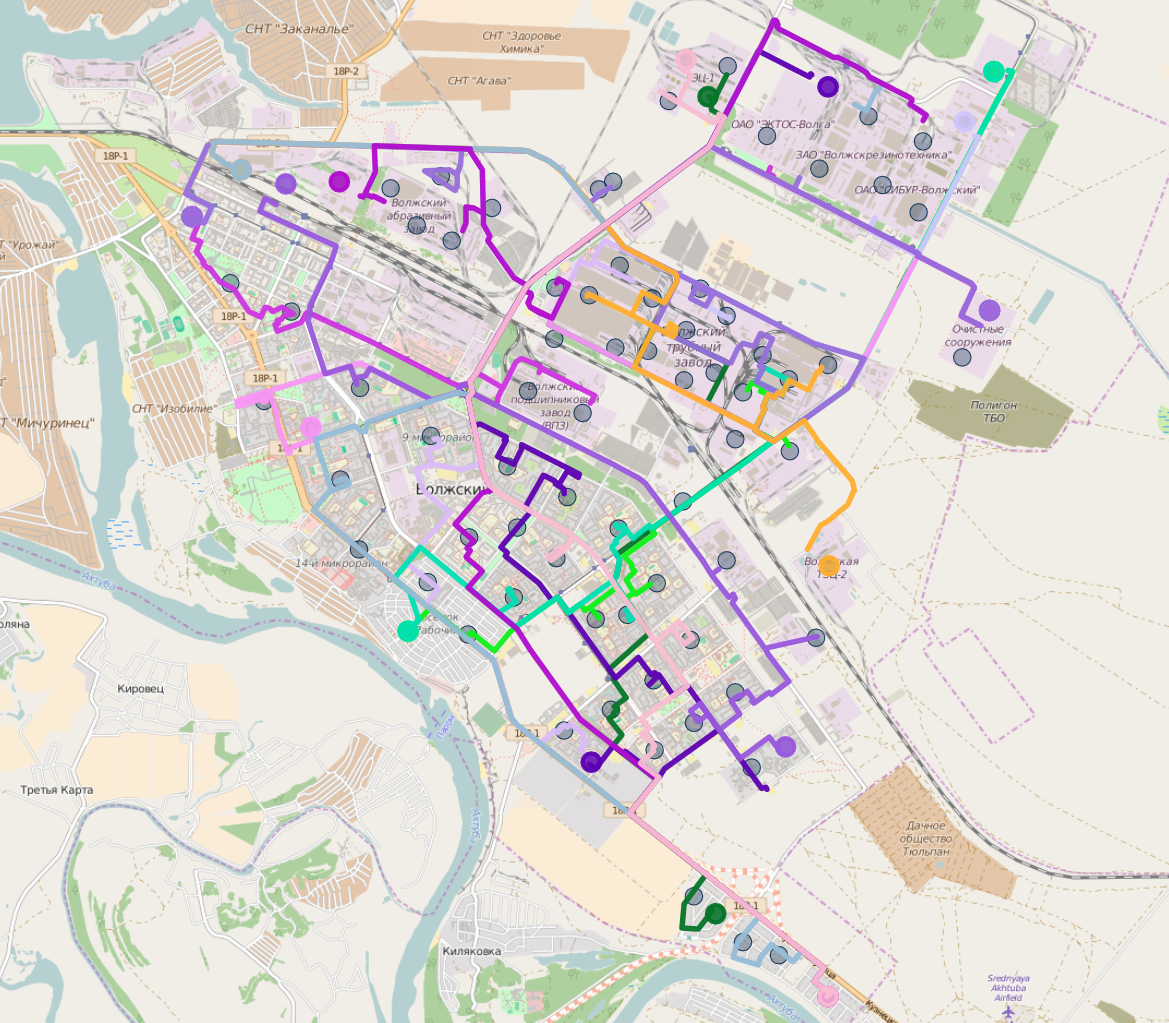
\includegraphics[width=0.7\textwidth]{100-14}
    \end{figure}
    \url{http://vstu-cad-stuff.github.io/routing/geojson/}
\end{frame}

\begin{frame}
    \frametitle{Основные результаты работы}
    В ходе проведения научной работы были получены следующие результаты:
    \begin{itemize}
        \item рассмотрены системы используемые для анализа транспортной сети;
        \item изучены алгоритмы используемые для задачи построения маршрута;
        \item предложен алгоритм формирования маршрутной сети на основе обработки данных о предпочтении;
        \item реализован алгоритм формирования маршрутной сети на основе обработки данных о предпочтении;
        \item проверена эффективность трёх стратегий реализованного алгоритма на сгенерированном наборе 
            данных;
    \end{itemize}
\end{frame}

\begin{frame}
    \frametitle{Публикации}
    \scriptsize
    \begin{thebibliography}{10}
        \bibitem{first} Strategway: web solutions for building public transportation routes using big geodata 
            analysis / Golubev A., Chechetkin I., Solnushkin K.S., Sadovnikova N., Parygin D., Shcherbakov M., 
            Brebels A. // Proceedings of The 17th International Conference on Information Integration and 
            Web-based Applications \& Services (iiWAS2015) (December 11 - 13, 2015 Brussels, Belgium) 
            ACM New York, New York pp. 665 - 668
        \bibitem{second} Комплекс инструментов интеллектуального анализа данных strategway для поддержки 
            принятия решений по управлению развитием инфраструктуры города / Садовникова Н.П., Щербаков М.В., 
            Парыгин Д.С., Солнушкин К.С., Голубев А.В., Чечёткин И.А. // В сборнике: Развитие средних 
            городов: замысел, модели, практика Материалы III Международной научно-практической конференции. 
            Волгоград, 2015. С. 147-150
        \bibitem{third} Автоматизация поддержки принятия решений по разработке маршрутов общественного 
            транспорта на основе анализа данных о корреспонденциях жителей / М. В. Щербаков, 
            Н. П. Садовникова, Д. С. Парыгин, А. В. Голубев, И. А. Чечеткин // Вестник компьютерных и 
            информационных технологий. -- М. : Издательский дом <<Спектр>>, 2016. -- В печати.
        \bibitem{fourth} Maxim Shcherbakov and Alexey Golubev, An algorithm for initial public transport 
            network design over geospatial data // 2016 IEEE International Smart Cities Conference (ISC2) 
            (ISC2 2016) (September, 2016 Trento, Italy) -- На рассмотрении.
    \end{thebibliography}
\end{frame}

\begin{frame}
    \frametitle{Вопросы}
    \begin{minipage}{0.3\textwidth}
        \begin{figure}[ht!]
            \centering
            
\includegraphics[width=\textwidth]{questions}
        \end{figure}
    \end{minipage}
    \begin{minipage}{0.6\textwidth}
        \begin{center}
            Голубев Алексей Владимирович, САПР-2п1,
            \href{mailto:ax.golubev@gmail.com}{ax.golubev@gmail.com}
        \end{center}
    \end{minipage}
\end{frame}